\documentclass[aspectratio=43]{beamer}
% \documentclass[handout]{beamer}
\usepackage[utf8]{inputenc}
\usepackage{multicol}
\usepackage{tikz} % drawings
\usepackage{animate} % animations
\usepackage{hyperref}
\usepackage{macros}

\usetikzlibrary{positioning, arrows}

\graphicspath{{img/}} % add the img folder to graphics path

\title{Hello \qw}
\date{November, 2018}
\author[Ramalho]{Miguel Sozinho Ramalho}
% \institution[FEUP]{Faculty of Engineering of the University of Porto}


%%%%%%%%%%%%%%%%%%%%%%%% THEME
\usetheme{material}
\useLightTheme
\usePrimaryTeal
\useAccentGreen

\usepackage{pgfpages}
% \setbeameroption{show notes}
% \setbeameroption{show notes on second screen=right}

\begin{document}

\begin{frame}
	\titlepage
\end{frame}


\begin{frame}{Table of contents}
	\begin{card}
		\tableofcontents
	\end{card}
\end{frame}

% Topics
% Theory
% Exercises explanation
% Conclusion
% References and additional sources

\section{Motivation}
\begin{frame}{Motivation}
\begin{card}[Why]
    \begin{chapquote}[2pt]{\href{https://en.wikipedia.org/wiki/Seth_Lloyd}{Seth Lloyd}}
        ``Classical computation is like a solo voice - one line of pure tones succeeding each other. Quantum computation is like a symphony - many lines of tones interfering with one another.''
    \end{chapquote}
\end{card}

\pagenumber
\end{frame}

\begin{frame}{Motivation}
\begin{card}[How]
    \qc can be seen as leveraging the phenomena that happen at the atomic and subatomic levels - in the \qw\xspace- to produce computations that, ultimately, surpass \cc.
\end{card}
\pagenumber
\end{frame}

\begin{frame}{About this course}
\begin{card}
    This course is suited for beginners in \qm and \qc. If you are already familiar with the concepts of a given week, you are encouraged to move forward in the course.

    This course brings novelty in that it focuses on \textbf{learning by doing}, and that is why you will also learn about \qk and \ibmqe.

    The author believes both that learning should be fun and that derision is a wonderful attention gripper, so humour will be used as the powerful tool that it is.
\end{card}
\pagenumber
\end{frame}

\begin{frame}{About this course - Study plan}
\begin{card}
    \begin{itemize}
        \item \qm 101
        \item \qk and \ibmq
        \item \qi
        \item Designing \qcts
        \item \qa
        \item \qc applications
        \item \q Computers - state of the art
        \item History, implications and ethics
    \end{itemize}
\end{card}
\pagenumber
\end{frame}

\section{\qp vs \cp}

\begin{frame}{\cp}
\begin{card}
    \cp (also \cm) describes the world \textit{as we see it}, in its macro level. Some of its properties:
    \begin{description}
        \item[size] objects with $size \gtrsim 1nm\ (10^{-9}m)$
        \item[speed] objects of $speed \lesssim \speedoflight$
        \item[causality] knowledge of the past allows calculation of the future (and \textit{vice versa})
    \end{description}
\end{card}
\pagenumber
\end{frame}


\begin{frame}{\qp}
\begin{card}
    \qp (also \qm) describes the world \textit{as we see it}, in its macro level. Some of its properties:
    \begin{description}
        \item[size] objects with $size \lesssim 1nm$
        \item[speed] objects of $speed \lesssim \speedoflight$
        \item[causality] knowledge of the past allows calculation of the future (and vice-versa)
    \end{description}
\end{card}
\pagenumber
\end{frame}

\begin{frame}{The kingdoms of \cl and \qm}
\begin{card}
    \centering\cardImg{classical_vs_quantum_dimensions.png}{\textwidth}
\end{card}
\pagenumber
\end{frame}

\section{Principles of \qm}
\subsubsection{\qsp}
\begin{frame}{\qsp}
    \begin{card}
        A \q state (of a particle) can be considered as being composed by more than one different states, simultaneously. It is not in state A \textbf{or} B, it is in state A \textbf{and} state B, at the same time. This defies classical views of the world, where two things are never true at the same time and requires some mental effort!\\
        The state is, therefore, in a kind of superposition.
    \end{card}
\pagenumber
\end{frame}

\begin{frame}{\qsp - Schrödinger's cat}
    \textbf{Thought experiment:} Imagine a cat locked inside a box, along with a poison releasing mechanism. The mechanism has a 50\% chance of having been activated at the time the box is about to be opened. At that moment, we cannot be sure of the cat's living state. Perhaps, we should assume the cat is both dead and alive, at the same time. With each state having the same probability.
    \begin{center}
	    \cardImg{img/cat.png}{0.5\textwidth}
    \end{center}
    \begin{center}
        To worlds, inside one.
    \end{center}
\pagenumber
\end{frame}


\begin{frame}{\qsp}
    \begin{cardTiny}
        Formally, such states are represented using the \textbf{Ket notation} (as defined by \textit{Paul Dirac}). State 0 would be \ket{0}.
    \end{cardTiny}
    \begin{cardTiny}
        \begin{multicols}{2}
    		Consider the electron of a Hydrogen atom, orbiting around the nucleus, with only two (simplification) possible energy states. As this is a \q particle, these energy states are quantized, that is, they take only discrete (quantified) values.
    		\centering
    		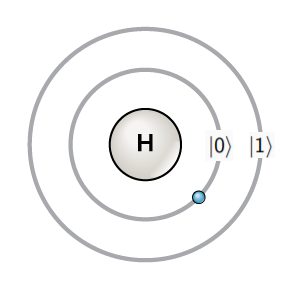
\includegraphics[width=0.4\textwidth]{hydrogen}
	    \end{multicols}
    \end{cardTiny}
\pagenumber
\end{frame}

\begin{frame}{\qsp}
    \begin{card}
        When we have no evidence of the electron's state, we assume that it is in a superposition of both positions. This \qsp $\ket{\delta}$ is written as:
	\begin{equation*}
	    \superpos[\delta]
	\end{equation*}
    \end{card}
    \begin{cardTiny}
        $\alpha$ and $\beta$ represent how likely each of the two states is. These are complex numbers such that $\sqrt{|\alpha|^2 + |\beta|^2} = 1$.
    \end{cardTiny}
\pagenumber
\end{frame}


\subsubsection{\qmt}
\begin{frame}{\qmt}
    \begin{cardTiny}
        From a pragmatic perspective, what happens when we open the box and look at the cat? From that moment on, only one state remains, either death \textbf{or} life. And we cannot close the box again and expect a different outcome.
    \end{cardTiny}
    \begin{cardTiny}
        \centering\textit{The cat is out of the box.}
    \end{cardTiny}
    \begin{cardTiny}
        A \textbf{Measurement} causes the system to stabilise, in a non-reversible way. When we perform a measurement  on the electron's state (let this process be a technicality, for now), we get $\ket{0}$ \textbf{or} $\ket{1}$. If we repeat the measurement, the result will be the same, \textbf{always}. Why? We don't know :)
    \end{cardTiny}
\pagenumber
\end{frame}

\section{References}
\begin{frame}{Where to learn more?}
\begin{card}
    \begin{itemize}
        \item \href{https://www.khanacademy.org/science/physics/quantum-physics/quantum-numbers-and-orbitals/a/the-quantum-mechanical-model-of-the-atom}{Khan Academy, The quantum mechanical model of the atom}
        \item \href{https://www.goodreads.com/book/show/331680.Programming_the_Universe}{Programming the Universe: A Quantum Computer Scientist Takes on the Cosmos}
        \item \href{https://www.goodreads.com/book/show/260142.The_Principles_of_Quantum_Mechanics}{The Principles of Quantum Mechanics, \textit{Paul Dirac}}
    \end{itemize}
\end{card}
\end{frame}

\end{document}
